% begin module improper-integral-type1-ex1
\begin{frame}
\begin{example}[Example 1, p. 545]
Determine whether $\int_1^\infty (1/x) \diff x$ is convergent or divergent.
\begin{columns}[c]
\column{.4\textwidth}
\ 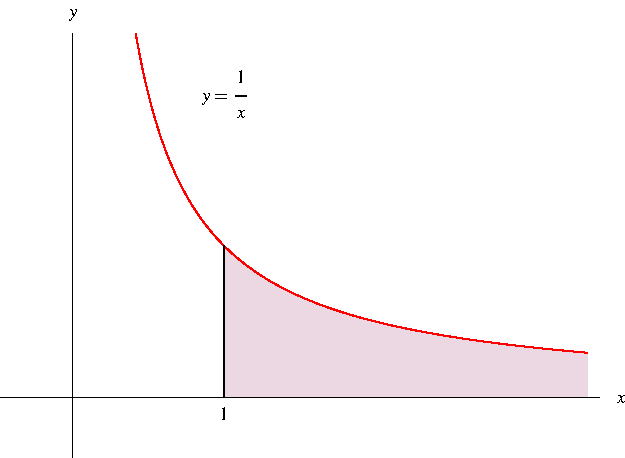
\includegraphics[height=3cm]{improper-integrals/pictures/08-08-ex1b.pdf}%

%\begin{center}
\uncover<7->{Infinite area}%
%\end{center}

\ \uncover<8->{%
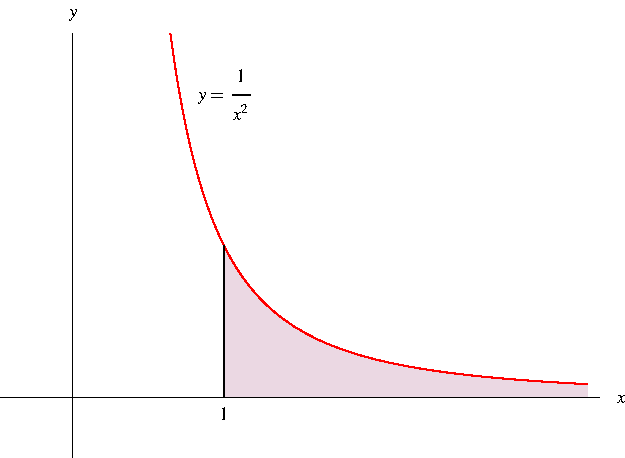
\includegraphics[height=3cm]{improper-integrals/pictures/08-08-ex1a.pdf}%
}%

%\begin{center}
\uncover<8->{Finite area}%
%\end{center}
\column{.6\textwidth}
\begin{eqnarray*}
\uncover<2->{%
\int_1^\infty \frac{1}{x}\diff x%
}%
& \uncover<2->{ = } & %
\uncover<2->{%
\lim_{t\rightarrow \infty} \int_1^t \frac{1}{x}\diff x%
}\\%
& \uncover<3->{ = } & %
\uncover<3->{%
\lim_{t\rightarrow \infty} \left[ \ln x\right]_1^t%
}\\%
& \uncover<4->{ = } & %
\uncover<4->{%
\lim_{t\rightarrow \infty} (\ln t - \ln 1)%
}\\%
& \uncover<5->{ = } & %
\uncover<5->{%
\lim_{t\rightarrow \infty} \ln t%
}%
\uncover<6->{ = \infty }%
\end{eqnarray*}
\uncover<7->{Therefore the improper integral is divergent.}
\end{columns}
\end{example}
\end{frame}
% end module improper-integral-type1-ex1
